% Created by tikzDevice version 0.12.6 on 2026-05-15 12:03:01
% !TEX encoding = UTF-8 Unicode
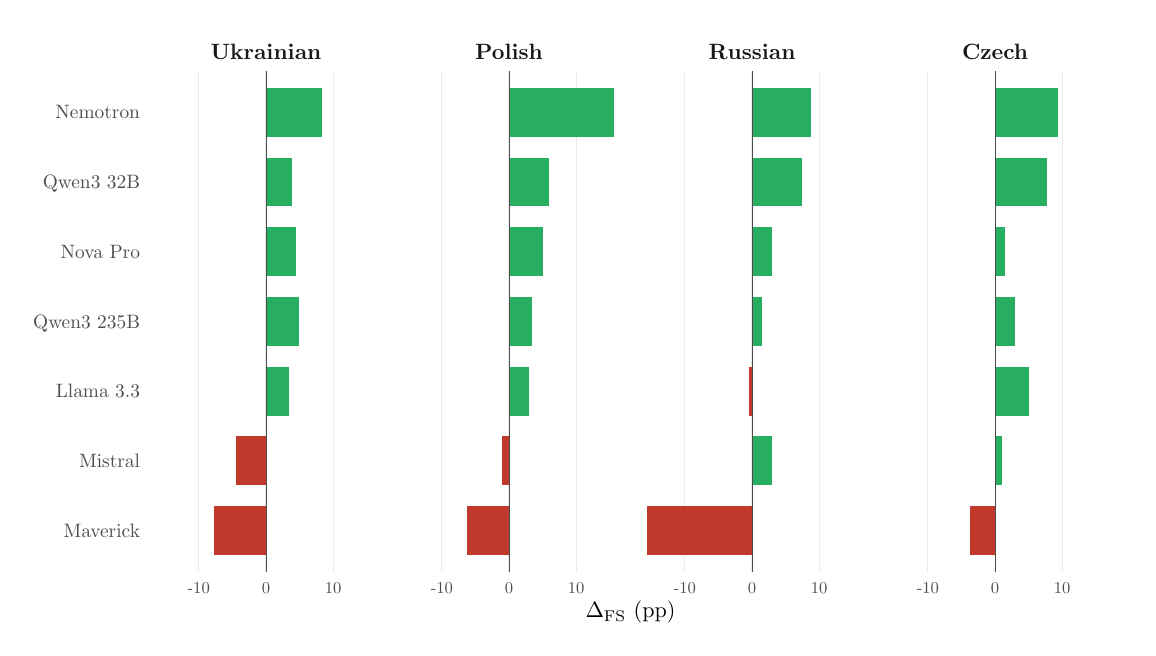
\begin{tikzpicture}[x=1pt,y=1pt]
\definecolor{fillColor}{RGB}{255,255,255}
\path[use as bounding box,fill=fillColor,fill opacity=0.00] (0,0) rectangle (397.48,216.81);
\begin{scope}
\path[clip] (  0.00,  0.00) rectangle (397.48,216.81);
\definecolor{fillColor}{RGB}{255,255,255}

\path[fill=fillColor] (  0.00,  0.00) rectangle (397.48,216.81);
\end{scope}
\begin{scope}
\path[clip] ( 44.19, 19.96) rectangle (128.01,201.33);
\definecolor{drawColor}{gray}{0.92}

\path[draw=drawColor,line width= 0.4pt,line join=round] ( 61.83, 19.96) --
	( 61.83,201.33);

\path[draw=drawColor,line width= 0.4pt,line join=round] ( 86.10, 19.96) --
	( 86.10,201.33);

\path[draw=drawColor,line width= 0.4pt,line join=round] (110.37, 19.96) --
	(110.37,201.33);
\definecolor{fillColor}{RGB}{192,57,43}

\path[fill=fillColor] ( 67.17, 26.26) rectangle ( 86.10, 43.89);
\definecolor{fillColor}{RGB}{39,174,96}

\path[fill=fillColor] ( 86.10, 76.64) rectangle ( 94.35, 94.28);
\definecolor{fillColor}{RGB}{192,57,43}

\path[fill=fillColor] ( 75.42, 51.45) rectangle ( 86.10, 69.08);
\definecolor{fillColor}{RGB}{39,174,96}

\path[fill=fillColor] ( 86.10,177.40) rectangle (106.24,195.04);

\path[fill=fillColor] ( 86.10,127.02) rectangle ( 96.78,144.66);

\path[fill=fillColor] ( 86.10,101.83) rectangle ( 97.99,119.47);

\path[fill=fillColor] ( 86.10,152.21) rectangle ( 95.56,169.85);
\definecolor{drawColor}{gray}{0.30}

\path[draw=drawColor,line width= 0.3pt,line join=round] ( 86.10, 19.96) -- ( 86.10,201.33);
\end{scope}
\begin{scope}
\path[clip] (132.01, 19.96) rectangle (215.84,201.33);
\definecolor{drawColor}{gray}{0.92}

\path[draw=drawColor,line width= 0.4pt,line join=round] (149.66, 19.96) --
	(149.66,201.33);

\path[draw=drawColor,line width= 0.4pt,line join=round] (173.92, 19.96) --
	(173.92,201.33);

\path[draw=drawColor,line width= 0.4pt,line join=round] (198.19, 19.96) --
	(198.19,201.33);
\definecolor{fillColor}{RGB}{192,57,43}

\path[fill=fillColor] (158.63, 26.26) rectangle (173.92, 43.89);
\definecolor{fillColor}{RGB}{39,174,96}

\path[fill=fillColor] (173.92, 76.64) rectangle (181.20, 94.28);
\definecolor{fillColor}{RGB}{192,57,43}

\path[fill=fillColor] (171.50, 51.45) rectangle (173.92, 69.08);
\definecolor{fillColor}{RGB}{39,174,96}

\path[fill=fillColor] (173.92,177.40) rectangle (212.03,195.04);

\path[fill=fillColor] (173.92,127.02) rectangle (186.30,144.66);

\path[fill=fillColor] (173.92,101.83) rectangle (182.18,119.47);

\path[fill=fillColor] (173.92,152.21) rectangle (188.24,169.85);
\definecolor{drawColor}{gray}{0.30}

\path[draw=drawColor,line width= 0.3pt,line join=round] (173.92, 19.96) -- (173.92,201.33);
\end{scope}
\begin{scope}
\path[clip] (219.84, 19.96) rectangle (303.66,201.33);
\definecolor{drawColor}{gray}{0.92}

\path[draw=drawColor,line width= 0.4pt,line join=round] (237.48, 19.96) --
	(237.48,201.33);

\path[draw=drawColor,line width= 0.4pt,line join=round] (261.75, 19.96) --
	(261.75,201.33);

\path[draw=drawColor,line width= 0.4pt,line join=round] (286.02, 19.96) --
	(286.02,201.33);
\definecolor{fillColor}{RGB}{192,57,43}

\path[fill=fillColor] (223.65, 26.26) rectangle (261.75, 43.89);

\path[fill=fillColor] (260.54, 76.64) rectangle (261.75, 94.28);
\definecolor{fillColor}{RGB}{39,174,96}

\path[fill=fillColor] (261.75, 51.45) rectangle (268.79, 69.08);

\path[fill=fillColor] (261.75,177.40) rectangle (283.11,195.04);

\path[fill=fillColor] (261.75,127.02) rectangle (269.03,144.66);

\path[fill=fillColor] (261.75,101.83) rectangle (265.39,119.47);

\path[fill=fillColor] (261.75,152.21) rectangle (279.71,169.85);
\definecolor{drawColor}{gray}{0.30}

\path[draw=drawColor,line width= 0.3pt,line join=round] (261.75, 19.96) -- (261.75,201.33);
\end{scope}
\begin{scope}
\path[clip] (307.66, 19.96) rectangle (391.48,201.33);
\definecolor{drawColor}{gray}{0.92}

\path[draw=drawColor,line width= 0.4pt,line join=round] (325.30, 19.96) --
	(325.30,201.33);

\path[draw=drawColor,line width= 0.4pt,line join=round] (349.57, 19.96) --
	(349.57,201.33);

\path[draw=drawColor,line width= 0.4pt,line join=round] (373.84, 19.96) --
	(373.84,201.33);
\definecolor{fillColor}{RGB}{192,57,43}

\path[fill=fillColor] (340.35, 26.26) rectangle (349.57, 43.89);
\definecolor{fillColor}{RGB}{39,174,96}

\path[fill=fillColor] (349.57, 76.64) rectangle (361.71, 94.28);

\path[fill=fillColor] (349.57, 51.45) rectangle (352.00, 69.08);

\path[fill=fillColor] (349.57,177.40) rectangle (372.14,195.04);

\path[fill=fillColor] (349.57,127.02) rectangle (353.21,144.66);

\path[fill=fillColor] (349.57,101.83) rectangle (356.61,119.47);

\path[fill=fillColor] (349.57,152.21) rectangle (368.50,169.85);
\definecolor{drawColor}{gray}{0.30}

\path[draw=drawColor,line width= 0.3pt,line join=round] (349.57, 19.96) -- (349.57,201.33);
\end{scope}
\begin{scope}
\path[clip] ( 44.19,201.33) rectangle (128.01,214.81);
\definecolor{drawColor}{gray}{0.10}

\node[text=drawColor,anchor=base,inner sep=0pt, outer sep=0pt, scale=  0.80] at ( 86.10,205.31) {\bfseries Ukrainian};
\end{scope}
\begin{scope}
\path[clip] (132.01,201.33) rectangle (215.84,214.81);
\definecolor{drawColor}{gray}{0.10}

\node[text=drawColor,anchor=base,inner sep=0pt, outer sep=0pt, scale=  0.80] at (173.92,205.31) {\bfseries Polish};
\end{scope}
\begin{scope}
\path[clip] (219.84,201.33) rectangle (303.66,214.81);
\definecolor{drawColor}{gray}{0.10}

\node[text=drawColor,anchor=base,inner sep=0pt, outer sep=0pt, scale=  0.80] at (261.75,205.31) {\bfseries Russian};
\end{scope}
\begin{scope}
\path[clip] (307.66,201.33) rectangle (391.48,214.81);
\definecolor{drawColor}{gray}{0.10}

\node[text=drawColor,anchor=base,inner sep=0pt, outer sep=0pt, scale=  0.80] at (349.57,205.31) {\bfseries Czech};
\end{scope}
\begin{scope}
\path[clip] (  0.00,  0.00) rectangle (397.48,216.81);
\definecolor{drawColor}{gray}{0.30}

\node[text=drawColor,anchor=base,inner sep=0pt, outer sep=0pt, scale=  0.60] at ( 61.83, 12.23) {-10};

\node[text=drawColor,anchor=base,inner sep=0pt, outer sep=0pt, scale=  0.60] at ( 86.10, 12.23) {0};

\node[text=drawColor,anchor=base,inner sep=0pt, outer sep=0pt, scale=  0.60] at (110.37, 12.23) {10};
\end{scope}
\begin{scope}
\path[clip] (  0.00,  0.00) rectangle (397.48,216.81);
\definecolor{drawColor}{gray}{0.30}

\node[text=drawColor,anchor=base,inner sep=0pt, outer sep=0pt, scale=  0.60] at (149.66, 12.23) {-10};

\node[text=drawColor,anchor=base,inner sep=0pt, outer sep=0pt, scale=  0.60] at (173.92, 12.23) {0};

\node[text=drawColor,anchor=base,inner sep=0pt, outer sep=0pt, scale=  0.60] at (198.19, 12.23) {10};
\end{scope}
\begin{scope}
\path[clip] (  0.00,  0.00) rectangle (397.48,216.81);
\definecolor{drawColor}{gray}{0.30}

\node[text=drawColor,anchor=base,inner sep=0pt, outer sep=0pt, scale=  0.60] at (237.48, 12.23) {-10};

\node[text=drawColor,anchor=base,inner sep=0pt, outer sep=0pt, scale=  0.60] at (261.75, 12.23) {0};

\node[text=drawColor,anchor=base,inner sep=0pt, outer sep=0pt, scale=  0.60] at (286.02, 12.23) {10};
\end{scope}
\begin{scope}
\path[clip] (  0.00,  0.00) rectangle (397.48,216.81);
\definecolor{drawColor}{gray}{0.30}

\node[text=drawColor,anchor=base,inner sep=0pt, outer sep=0pt, scale=  0.60] at (325.30, 12.23) {-10};

\node[text=drawColor,anchor=base,inner sep=0pt, outer sep=0pt, scale=  0.60] at (349.57, 12.23) {0};

\node[text=drawColor,anchor=base,inner sep=0pt, outer sep=0pt, scale=  0.60] at (373.84, 12.23) {10};
\end{scope}
\begin{scope}
\path[clip] (  0.00,  0.00) rectangle (397.48,216.81);
\definecolor{drawColor}{gray}{0.30}

\node[text=drawColor,anchor=base east,inner sep=0pt, outer sep=0pt, scale=  0.70] at ( 40.59, 32.67) {Maverick};

\node[text=drawColor,anchor=base east,inner sep=0pt, outer sep=0pt, scale=  0.70] at ( 40.59, 57.86) {Mistral};

\node[text=drawColor,anchor=base east,inner sep=0pt, outer sep=0pt, scale=  0.70] at ( 40.59, 83.05) {Llama 3.3};

\node[text=drawColor,anchor=base east,inner sep=0pt, outer sep=0pt, scale=  0.70] at ( 40.59,108.24) {Qwen3 235B};

\node[text=drawColor,anchor=base east,inner sep=0pt, outer sep=0pt, scale=  0.70] at ( 40.59,133.43) {Nova Pro};

\node[text=drawColor,anchor=base east,inner sep=0pt, outer sep=0pt, scale=  0.70] at ( 40.59,158.62) {Qwen3 32B};

\node[text=drawColor,anchor=base east,inner sep=0pt, outer sep=0pt, scale=  0.70] at ( 40.59,183.81) {Nemotron};
\end{scope}
\begin{scope}
\path[clip] (  0.00,  0.00) rectangle (397.48,216.81);
\definecolor{drawColor}{RGB}{0,0,0}

\node[text=drawColor,anchor=base,inner sep=0pt, outer sep=0pt, scale=  0.80] at (217.84,  3.56) {$\Delta_{\mathrm{FS}}$ (pp)};
\end{scope}
\end{tikzpicture}
